\documentclass[11pt,a4paper]{article}

\usepackage{style2017}
\usepackage{hyperref}
\usepackage{colortbl}

\hypersetup{
    colorlinks =false,
    linkcolor=blue,
   linkbordercolor = 1 0 0
}
\renewcommand\arraystretch{1.6}
\newcounter{numexo}
\setcellgapes{1pt}

\begin{document}



%\begin{NSI}
%{Activité}{Protocole de routage}
%\end{NSI}

\begin{huge}
\textbf{Activité : } Protocole de routage
\end{huge}\medskip
\hrule


\section*{Passerelle et interface}

Les routeurs disposent de plusieurs \textbf{interfaces} réseaux qui permettent aux routeurs de communiquer entre eux. Les interfaces sont désignées par leur nom ou par leur adresse IP. \medskip

Une \textbf{passerelle} est une interface du routeur qui permet d'accéder au réseau de destination.\medskip

Le réseau représenté ci-dessous permet de relier 2 réseaux désignés par L1 et L2. 

\begin{center}
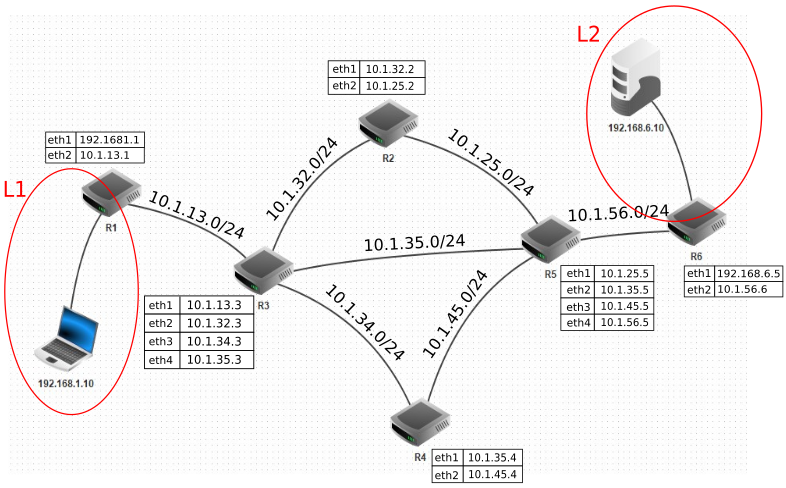
\includegraphics[scale=0.8]{img/reseau_complet.eps}
\end{center}


\begin{enumerate}
\item Quelles sont les interfaces du routeur R1 ?

Le routeur R1 a 2 interfaces réseau \textbf{eth1} et \textbf{eth2}.
\vfill

\item Quelle est l'interface du routeur R1 pour accéder au réseau L2 ?

L'interface du routeur R1 qui permet d'accéder au réseau L2 est \textbf{eth2}.
\vfill

\item Quelle est la passerelle suivante du routeur R1 pour accéder au réseau L2 ?

La passerelle qui permet au routeur R1 d'accéder au réseau L2 est l'interface du routeur R3 d'adresse IP 10.1.13.3
\vfill

\item Quelles sont les interfaces du routeur R3 ?

Le routeur R3 dispose de 4 interfaces : \textbf{eth1}, \textbf{eth2}, \textbf{eth3} et \textbf{eth4}.
\vfill
\item Le routeur R3 envoie les paquets vers le routeur R5. 

Quelle est l'interface utilisée pour accéder au réseau L2 ? Quelle est la passerelle suivante ?

L'interface eth4 du routeur R3 est utilisée pour envoyer les paquets au réseau L2.

La passerelle suivante est l'interface eth2 du routeur R5 d'adresse IP 10.1.35.5
\vfill

\item Un utilisateur du portable du réseau L1 se connecte sur le serveur du réseau L2. 

Quelle est la passerelle renseignée sur le portable ?

La passerelle indiquée sur le portable est l'adresse IP de l'interface \textbf{eth1} du routeur R1, soit 192.168.1.1.
\vfill

\end{enumerate}

\newpage

\section*{Table de routage}

Les routeurs déterminent à l'aide d'algorithmes un parcours pour atteindre le réseau de destination. Ces algorithmes optimisent les parcours, notamment lorsque le réseau est modifié suite à une panne ou une transformation. 

Les routes sont inscrites dans des \textbf{tables de routage} mise à jour régulièrement et contenant les informations suivantes:

\begin{center}
\begin{tabular}{*{3}{|C{4cm}}|}\hline
\textbf{réseau destination} & \textbf{passerelle suivante} & \textbf{interface} \\\hline
\end{tabular}
\end{center}



\begin{enumerate}
\item On donne la table de routage du routeur R1. Compléter les cases vides avec les bonnes valeurs.

\begin{center}
\begin{tabular}{*{3}{|C{4cm}}|}\hline
\textbf{réseau destination} & \textbf{passerelle suivante} & \textbf{interface} \\\hline
192.168.1.0/24 & 192.168.1.1 & eth1  \\\hline
10.1.13.0/24 & 10.1.13.1 & eth2 \\\hline
\end{tabular}
\end{center}

\item On donne la table de routage du routeur R3. Compléter les cases vides avec les bonnes valeurs.

\begin{center}
\begin{tabular}{*{3}{|C{4cm}}|}\hline
\textbf{réseau destination} & \textbf{passerelle suivante} & \textbf{interface} \\\hline
10.1.13.0/24 & 10.1.13.3 & eth1 \\\hline
10.1.32.0/24 & 10.1.32.3 & eth2 \\\hline
10.1.34.0/24 & 10.1.34.3 & eth3 \\\hline
10.1.35.0/24 & 10.1.35.3 & eth4 \\\hline
192.168.1.0/24 & 10.1.13.1 & eth1 \\\hline
192.168.6.0/24 & 10.1.35.5 & eth4 \\\hline
\end{tabular}
\end{center}
Que peut-on dire concernant la dernière route de la table ?

Il existe plusieurs routes pour accéder au réseau d'adresse 192.168.6.0/24 depuis le routeur R3. On aurait pu écrire choisir l'interface eth2 et la passerelle 10.1.32.2 \bigskip

\item Compléter la table de routage du routeur R6.

\begin{center}
\begin{tabular}{*{3}{|C{4cm}}|}\hline
\textbf{réseau destination} & \textbf{passerelle suivante} & \textbf{interface} \\\hline
10.1.56.0/24 & 10.1.56.6 & eth2 \\\hline
192.168.6.0/24 & 192.168.6.5 & eth1 \\\hline
192.168.1.0/24 & 10.1.56.5 & eth2 \\\hline
10.1.35.0/24 & 10.1.56.5 & eth2 \\\hline
 & &  \\\hline
0.0.0.0/24 & 10.1.56.5 & eth2 \\\hline
\end{tabular}
\end{center}

La dernière ligne indique que pour tout les autre réseaux, l'interface est eth2 et la passerelle est 10.1.56.5
\end{enumerate}


\newpage


\section*{Protocoles}

La communication entre machines repose sur des protocoles. Il existe plusieurs protocoles concernant les routeurs. On va en étudier 2 : \textbf{RIP} et \textbf{OSPF}.


\subsection*{Protocole RIP}

Le protocole RIP détermine la meilleure route entre 2 réseaux en mémorisant le nombre de routeurs à traverser pour parvenir au réseau de destination. Cette quantité de routeurs à traverser est appelée \textbf{distance} ou \textbf{métrique}. Cette métrique est enregistrée dans la table de routage.


\begin{enumerate}
\item On donne la table de routage du routeur R1. Compléter les cases vides avec les bonnes valeurs.

\begin{center}
\begin{tabular}{*{4}{|C{4cm}}|}\hline
\textbf{réseau destination} & \textbf{passerelle suivante} & \textbf{interface}  & \textbf{distance / métrique} \\\hline
192.168.1.0/24 & 192.168.1.1 & eth 1 & 0\\\hline
10.1.13.0/24 & 10.1.13.1 & eth2 & 0 \\\hline
10.1.32.0/24 & 10.1.13.3 & eth2 &  1\\\hline
10.1.34.0/24 & 10.1.13.3 & eth2 & 1\\\hline
10.1.35.0/24 & 10.1.13.3 & eth2 & 1 \\\hline
10.1.56.0/24 & 10.1.13.3 & eth2 & 2 \\\hline
192.168.6.0/24 & 10.1.13.3 & eth2 & 3 \\\hline
\end{tabular}
\end{center}



\item On donne la table de routage du routeur R3. Compléter les cases vides avec les bonnes valeurs.

\begin{center}
\begin{tabular}{*{4}{|C{4cm}}|}\hline
\textbf{réseau destination} & \textbf{passerelle suivante} & \textbf{interface} & \textbf{distance / métrique} \\\hline
10.1.13.0/24 & 10.1.13.3 & eth1 & 0 \\\hline
10.1.32.0/24 & 10.1.32.3 & eth2 & 0 \\\hline
10.1.34.0/24 & 10.1.34.3 & eth3 & 0 \\\hline
10.1.35.0/24 & 10.1.35.3 & eth4 & 0 \\\hline
192.168.1.0/24 & 10.1.13.3 & eth1 & 1 \\\hline
192.168.6.0/24 & 10.1.35.5 & eth4 & 2  \\\hline
\end{tabular}
\end{center}


\item Compléter la table de routage du routeur R6.

\begin{center}
\begin{tabular}{*{4}{|C{4cm}}|}\hline
\textbf{réseau destination} & \textbf{passerelle suivante} & \textbf{interface} & \textbf{distance / métrique} \\\hline
10.1.56.0/24 & 10.1.56.6 & eth2 & 0 \\\hline
192.168.1.0/24 & 10.1.56.5 & eth2 & 3 \\\hline
\end{tabular}
\end{center}

\end{enumerate}
%\end{enumerate}

\newpage


\subsection*{Protocole OSPF}
Le protocole RIP ne tient pas compte du débit et de la distance entre les routeurs. De plus, les protocoles RIP ne sont pas adaptés pour les grands réseaux supérieurs à 15 sauts. Le protocole OSPF palie à ces problèmes.\medskip

Ce protocole permet de gérer de grands domaines et prend en compte les débits pour mesurer la rapidité d'une route, son \textbf{coût}. Le calcul du coût se fait avec la relation suivante :
$$\text{c} = \dfrac{10^8}{\text{d}}$$
où \textbf{c} est le coût et \textbf{d} le débit de la route en bits par seconde. A noter que le nombre $10^{8}$ est une constante liée au routeur et peut être différente.
\medskip

Pour simplifier le réseau, on le représente par un graphe:
\begin{itemize}
\item Chaque sommet du graphe représente un routeur;
\item Chaque arête du graphe représente un lien entre deux routeurs;
\item Le poids donné pour chaque arête indique le \textbf{coût} de communication entre 2 routeurs.
\end{itemize}

\begin{center}
\psset{unit=1cm}
\begin{pspicture}(10,6)
\cnodeput(0.5,3.5){R1}{R1}
\cnodeput(5.5,5.5){R2}{R2}
\cnodeput(2.5,3){R3}{R3}
\cnodeput(5,1){R4}{R4}
\cnodeput(7.5,3){R5}{R5}
\cnodeput(9.5,2.5){R6}{R6}
\ncline{R1}{R3}\ncput*{\bf ...}
\ncline{R3}{R2}\ncput*{\bf 4}
\ncline{R3}{R4}\ncput*{\bf 5}
\ncline{R3}{R5}\ncput*{\bf 6}
\ncline{R2}{R5}\ncput*{\bf 3}
\ncline{R4}{R5}\ncput*{\bf ...}
\ncline{R5}{R6}\ncput*{\bf 1}
\end{pspicture}
\end{center} 

\begin{enumerate}
\item Sachant que le débit entre les routeurs R1 et R2 est de 50 Mbits par seconde, calculer le coût de cette route.
\item Calculer le débit de la route qui relie les routeurs R3 et R4.
\item La communication entre les routeurs R4 et R5 est de 1Gb/s. Calculer son coût.
\item Quelle est la route qui est la plus rapide entre les routeurs R1 et R6 ?
\end{enumerate}

\end{document}
